\section{i numeri complessi}
%
%
%
\label{sec:complessi}

Dal punto di vista geometrico l'insieme $\CC$ dei \emph{numeri complessi}%
\mymargin{numeri complessi}%
\index{numeri!complessi}
\index{$\CC$}
può essere visto come una rappresentazione cartesiana 
del piano euclideo.
Sul piano fissiamo arbitrarimente un punto $0$ (l'origine) 
e fissiamo, arbitrariamente, una base $e_1$, $e_2$ di vettori ortonormali.
Identifichiamo ogni punto del piano con i corrispondenti vettori
applicati in $0$. La retta generata dal vettore $e_1$ la identifichiamo
con la retta $\RR$ dei numeri reali e quindi poniamo $1=e_1$.
La retta ortogonale generata dal vettore $e_2$ verrà chiamata
retta dei \emph{numeri immaginari} e definiamo $i=e_2$.

Un generico punto $z$ del piano $\CC$ potrà essere scritto in
maniera univoca nella base scelta: $z = x e_1 + y e_2$ ovvero,
per come abbiamo chiamato $e_1$ ed $e_2$:
\[
z = x + i y.
\]
Tale $z$ viene chiamato
\emph{numero complesso} con parte reale $x$ e parte immaginaria $y$.
Questa rappresentazione del numero complesso $z$ viene
chiamata \emph{rappresentazione cartesiana}%
\mymargin{rappresentazione cartesiana}%
\index{rappresentazione!cartesiana} in quanto definisce
il punto $z$ del piano complesso tramite le sue coordinate cartesiane
$x$ e $y$.
I numeri reali sono \emph{immersi} nei complessi, nel senso che se
$x\in \RR$ allora $z= x + i\cdot 0 = x$ è anche un numero complesso.
Il numero complesso $i = 0 + i\cdot 1$ viene chiamata \emph{unità immaginaria}%
\mymargin{unità immaginaria}%
\index{unità!immaginaria}
e i numeri complessi della forma $iy$ sono chiamati \emph{immaginari}.
\index{numeri!immaginari}
\index{immaginario}
Un numero
complesso $z = x+iy$ è quindi una somma tra un numero reale ed un numero
immaginario. Il numero reale $x$ viene chiamato \emph{parte reale}
\index{parte!reale}
di $z$ e
si denota con $x=\Re z$.
\mymargin{$\Re z$}%
\index{$\Re z$}
Il numero reale $y$ viene chiamato
\emph{parte immaginaria}
\index{parte!immaginaria}
di $z$ e si denota con $y=\Im z$
\mymargin{$\Im z$}%
\index{$\Im z$}
(osserviamo che la parte immaginaria di un numero complesso è un numero
reale, non immaginario). Dunque $z= \Re z + i \Im z$.

L'insieme $\CC$, per come
è stato costruito, è uno spazio vettoriale reale di dimensione $2$.
Abbiamo quindi già definite la \emph{addizione}%
\mymargin{addizione}%
\index{addizione}
\index{complessi!addizione}
tra elementi di $\CC$ e la moltiplicazione
tra elementi di $\CC$ ed elementi di $\RR$.
Se $a,b,c,d,t\in \RR$ si ha:
\begin{gather*}
 (a+ib) + (c+id) = (a+c) + i (b+d), \\
 t(a+ib) = ta + itb.
\end{gather*}

Vogliamo estendere la \emph{moltiplicazione}%
\mymargin{moltiplicazione}%
\index{moltiplicazione} a tutte le coppie di numeri complessi.
\index{complessi!moltiplicazione}
Imponendo (arbitrariamente) che valga $i\cdot i = -1$ e che rimanga
valida la proprietà distributiva, si ottiene
questa definizione:
\[
   (a+ib) \cdot (c+id) = (ac-bd) + i(ad+bc).
\]

Si può verificare che questa moltiplicazione estende quella ``scalare'' definita
in precedenza.
E' anche facile verificare che addizione e moltiplicazione soddisfano
le proprietà commutativa associativa e distributiva,
che $0$ è elemento neutro per la addizione, che $1$ è elemento neutro
della moltiplicazione.
Si osservi che se $z=x+iy$ non è nullo, allora
\[
  (x+iy) \cdot \frac{x-iy}{x^2+y^2} = 1.
\]
Significa che ogni $z\neq 0$ ammette inverso moltiplicativo e quindi $\CC$,
in definitiva,
risulta essere un campo.

Osserviamo che su $\CC$ non si definisce una relazione d'ordine perché
in effetti non è possibile definire un ordine ``compatibile'' con le operazioni
appena definite.%
\mynote{%
Se $\CC$ fosse un campo ordinato per assurdo
si dovrebbe avere,
che $z^2\ge 0$ per ogni $z\in \CC$ (questo è vero in tutti i campi ordinati). 
Ma
allora $-1 =i^2 \ge 0$ cioè $1\le 0$ che è in contraddizione
con la proprietà $0<1$ valida in ogni campo ordinato.
} % marginnote

Su $\CC$ definiamo delle ulteriori operazioni.
Il \emph{coniugato}%
\mymargin{coniugato}%
\index{coniugato}%
\index{complessi!coniugio}
di un numero complesso $z=x+iy$ è il numero
$\bar z = x - iy$. Geometricamente l'operazione di coniugio è una simmetria
rispetto alla retta reale. I numeri reali sono in effetti punti fissi del
coniugio (il coniugato di un numero reale è il numero stesso).
E' un semplice esercizio verificare che il coniugio ``attraversa''
somma e prodotto:
\[
\overline{z+w} = \bar z + \bar w, \qquad
\overline{z\cdot w} = \bar z \cdot \bar w.
\]
Ovviamente risulta $\overline {\bar z} = z$.
E' anche utile osservare che si ha:
\begin{equation}\label{eq:re_im}
  \Re z = \frac{z+\bar z}{2}, \qquad
  \Im z = \frac{z-\bar z}{2i}
\end{equation}
e
\[
z \cdot \bar z = (x+iy)(x-iy) = x^2-i^2y^2 = x^2+y^2.
\]

Possiamo allora definire il
\emph{modulo}%
\mymargin{modulo}%
\index{modulo}%
\index{complessi!modulo}
 di un numero complesso $z=x+iy$
come il numero reale
\[
\abs{z} = \sqrt{z\cdot\bar z} = \sqrt{x^2+y^2}.
\]
Geometricamente tale quantità rappresenta la distanza del punto $z$
dal punto $0$ e quindi la distanza tra due numeri complessi $z$ e
$w$ si potrà rappresentare con $\abs{z-w}$.

Osserviamo che se $z = x \in \RR \subset \CC$ il modulo di $z$ coincide
con il valore assoluto: $\abs{z} = \sqrt{x^2} = \abs{x}$ e per questo
motivo non distinguiamo, nelle notazioni, il modulo dal valore assoluto.
Più in generale risulta per ogni $z\in \CC$ (la verifica è immediata):
\[
  \abs{\Re z} \le \abs{z}, \qquad
  \abs{\Im z} \le \abs{z}.
\]

Possiamo a questo punto trovare una utile formula per calcolare
il reciproco di un numero complesso. Essendo infatti
$z\cdot \bar z = \abs{z}^2$ si osserva che
\[
  \frac{1}{z}
  = \frac{\bar z}{ \bar z \cdot z}
  = \frac{\bar z}{\abs{z}^2}.
\]

\begin{theorem}
Il modulo di un numero complesso soddisfa (come il valore assoluto)
le seguenti proprietà
\begin{enumerate}
\item $\big\lvert\abs{z}\big\rvert = \abs{z}$,
\item $\abs{-z} = \abs{z}$ = $\abs{\bar z}$,
\item $\abs{z\cdot w} = \abs{z}\cdot\abs{w}$.
\item $\abs{z+w} \le \abs{z}+\abs{w}$ (convessità),
\item $\abs{z-w} \le \abs{z-v} + \abs{v-w}$ (disuguaglianza triangolare),
\end{enumerate}
\end{theorem}
%
\begin{proof}
La prima proprietà è ovvia in quanto il valore assoluto di un numero reale
non negativo è il numero stesso.

La seconda proprietà viene immediatamente dalla definizione.

La terza proprietà si ottiene osservando che 
\[
\abs{z\cdot w}^2 
  = zw \cdot \overline{zw} 
  = z\bar z \cdot w\bar w = \abs{z}^2 \cdot \abs{w}^2 
  = (\abs z \cdot \abs w)^2.
\]
% Per la terza proprietà sia $z=x+iy$, $w=a+ib$.
% Allora:
% \begin{align*}
% \abs{z\cdot w}
% &= \abs{(x+iy)\cdot(a+ib)}
% =\abs{xa - y b+ i(xb + ay)} \\
% &= \sqrt{(xa-yb)^2 + (xb+ay)^2}\\
% &=\sqrt{x^2 a^2 + y^2b^2 - 2xayb + x^2b^2+a^2y^2+2xbay} \\
% &=\sqrt{x^2 a^2 + y^2 b^2 + x^2 b^2 + a^2 y^2}\\
% &=\sqrt{x^2(a^2+b^2) + y^2(a^2+b^2)}\\
% &=\sqrt{(x^2+y^2)(a^2+b^2)}
% =\abs{x+iy} \cdot \abs{a+ib}\\
% &=\abs{z}\cdot\abs{w}.
% \end{align*}

Per la quarta disuguaglianza osserviamo che si ha
\[
  \abs{z+w}^2 = (z+w)\cdot(\bar z + \bar w)
  = \abs{z}^2 + \abs{w}^2 + z\cdot \bar w + \bar z \cdot w
\]
e visto che
\[
  z\cdot \bar w + \bar z \cdot w
  = z \cdot \bar w + \overline{z \cdot \bar w}
  = 2 \Re(z\bar w)
  \le 2 \abs {z\bar w}
  = 2 \abs{z}\cdot\abs{\bar w}
  = 2 \abs{z}\cdot\abs{w}
\]
otteniamo
\[
 \abs{z+w}^2 \le \abs{z}^2+\abs{w}^2 + 2 \abs{z}\cdot\abs{w}
 =\enclose{\abs z + \abs w}^2
\]
che è equivalente alla disuguaglianza di convessità.

La disuguaglianza triangolare è equivalente alla convessità, infatti
\[
  \abs{z-w} = \abs{(z-v) + (v-w)}
  \le \abs{z-v} + \abs{v-w}.
\]
\end{proof}

\begin{figure}
  \begin{center}
    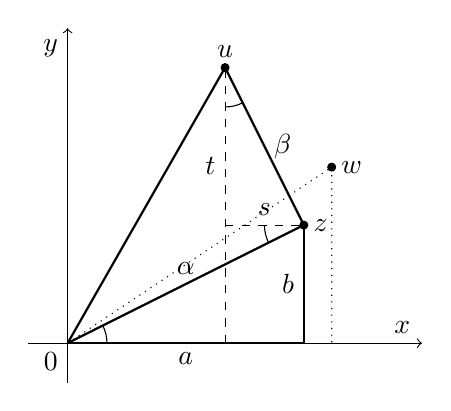
\begin{tikzpicture}[x=0.5cm,y=0.5cm]
    	\draw[->] (-1,0) -- (9,0);
      \draw[->] (0,-1) -- (0,8);
      %
      \draw[dotted] (0,0) -- ({sqrt(45)},{sqrt(20)}) -- ({sqrt(45)},0);
      \draw[fill] ({sqrt(45)},{sqrt(20)}) node[right] {$w$} circle [radius=0.1];
      %
      \draw[thick] (0,0) -- (6,0);
      \draw[thick] (0,0) -- (6,3);
      \draw[thick] (0,0) -- (4,7);
      \draw[thick] (6,0) -- (6,3);
      \draw[thick] (6,3) -- (4,7);
      %
      \draw[dashed] (4,0) -- (4,7);
      \draw[dashed] (4,3) -- (6,3);
      %
      \draw (1,0) arc (0:{atan(1/2)}:1);
      \draw (6,3)+(-1,0) arc (180:{180+atan(1/2)}:1);
      \draw (4,7)+(0,-1) arc (-90:{-90+atan(1/2)}:1);
      %
      \draw[fill] (6,3) node[right] {$z$} circle [radius=0.1];
      \draw[fill] (4,7) node[above] {$u$} circle [radius=0.1];
      %
      \node[below] at (3,0) {$a$};
      \node[left] at (6,1.5) {$b$};
      \node[above] at (3,1.5) {$\alpha$};
      \node[right] at (5,5) {$\beta$};
      \node[above] at (5,3) {$s$};
      \node[left] at (4,4.5) {$t$};
      \node[above] at (8.5,0) {$x$};
      \node[left] at (0,7.5) {$y$};
      \node[below left] at (0,0) {$0$};
    \end{tikzpicture}
  \end{center}
  \caption{Consideriamo i numeri complessi $z=a+ib$ e $w=\alpha+i\beta$
  e supponiamo che sia $\alpha^2 = a^2+b^2$.
  Si consideri il punto $u$ che si ottiene ruotando il punto $w$ dell'angolo
  individuato dal punto $z$. Si avrà allora $u=a-s + i(b+t)$ dove $s$ e $t$
  sono i cateti del triangolo rettangolo con ipotenusa $\beta$.
  Grazie alle proprietà di similitudine dei triangoli si ha
  $\frac{s}{\beta} = \frac{b}{\alpha}$ e $\frac{t}{\beta} = \frac{a}{\alpha}$
  da cui si ottiene quindi $u = a-\frac{b\beta}{\alpha}+i(b+\frac{a\beta}{\alpha})$
  ovvero $\alpha u = (a\alpha - b \beta) + i (b\alpha + a \beta) = z\cdot w$.
  Significa che il numero complesso $z\cdot w$ si trova sulla semiretta
  che individua un angolo che è la somma degli angoli individuati
  dai numeri complessi $z$ e $w$.
  }
  \label{fig:prodotto_complesso}
\end{figure}

Possiamo ora dare una interpretazione geometrica del prodotto $z\cdot w$
tra due numeri complessi. In primo luogo sappiamo che $\abs{z\cdot w} = \abs{z} \cdot \abs{w}$ e dunque il punto del piano che rappresenta il prodotto $z\cdot w$ si trova ad una distanza dall'origine che è pari al prodotto delle distanze
dei punti $z$ e $w$. Inoltre l'angolo individuato da $z\cdot w$ rispetto
all'asse delle $x$ positive risulta uguale alla somma
degli angoli individuati dai punti $z$ e $w$ come mostrato in figura~\ref{fig:prodotto_complesso}.

Anche il piano dei numeri complessi può essere esteso aggiungendoci
un punto all'\emph{infinito}%
\mymargin{infinito}%
\index{infinito}.
A differenza dei reali, su cui era presente un ordinamento che era utile conservare,
nel caso dei numeri complessi è più usuale utilizzare un unico punto infinito
che si denota con \emph{$\infty$}%
\mymargin{$\infty$}%
\index{$\infty$}.
Definiamo l'insieme dei complessi estesi $\bar \CC$ come
\[
\bar \CC = \CC \cup \ENCLOSE{\infty}.
\]
Definiamo
\begin{align*}
  z + \infty &= \infty \qquad \forall z \in \CC\\
  z - \infty &= \infty \qquad \forall z \in \CC\\
   z\cdot \infty &= \infty \qquad \forall z \in \bar\CC\setminus\ENCLOSE{0} \\
   z / \infty &= 0 \qquad \forall z \in \CC \\
   z / 0 &= \infty \qquad \forall z \in \bar \CC \setminus\ENCLOSE{0}\\
   \bar \infty &= \infty \\
   \abs{\infty} &= +\infty \in \bar \RR.
\end{align*}
Si noti che abbiamo definito la divisione per zero di numeri complessi
(e quindi anche reali) diversi da zero. Il risultato è $\infty$ e quindi
rimane confermato che la divisione per zero non è una operazione valida
se vogliamo un risultato finito.
Una quantità $z\in \bar \CC$ sarà detta \emph{finita} se $z\in \CC$.

\begin{example}
  La funzione $f\colon \bar \CC \to \bar \CC$ 
  definita da 
  \[
  f(z) = \frac{1}{z}
  \]
  è una funzione bigettiva di $\bar \CC$ in sé.
  Dal punto di vista geometrico il coniugato di tale funzione
  ovvero la funzione $z\mapsto \frac 1 {\bar z}$ 
  è l'inversione circolare rispetto al cerchio unitario di $\CC$:
  i punti sulla circonferenza unitaria vengono lasciati fissi,
  i punti all'interno vengono mandati all'esterno rimanendo sullo 
  stesso raggio uscente dall'origine e invertendo il proprio modulo.
  I punti $0$ e $\infty$ si scambiano.
\end{example}

%% % ancora non abbiamo definito il concetto di funzione continua
%% Per le funzioni di variabile complessa e/o a valori complessi 
%% si applica la stessa definizione~\ref{def:continua} di continuità 
%% che abbiamo dato per le funzioni reali utilizzando il modulo 
%% complesso al posto del valore assoluto.
%% \index{continuità!campo complesso}%
%% \index{funzione!continua!complessa}%

\begin{exercise}
  \label{ex:radice_uno}
Risolvere, in campo complesso, l'equazione 
\[
  z^2=1.
\]
\end{exercise}
\begin{proof}[Svolgimento.]
Posto $z=x+iy$ con $x,y\in \RR$, si ottiene 
$x^2-y^2 + 2 i xy = 1$ da cui, uguagliando parte reale 
e parte immaginaria, si ottiene $x^2-y^2=1$, $xy=0$.
Non può essere $x=0$ altrimenti si avrebbe $y^2=-1$
che non ha soluzione $y\in \RR$.
Dunque deve essere $y=0$ da cui si ottiene $x^2=1$ e quindi $x=+\pm 1$.

Dunque l'equazione ha due soluzioni: $z=1$ e $z=-1$.
\end{proof}
\begin{exercise}
  \label{ex:radice_quarta_uno}
Risolvere, in campo complesso, l'equazione
\[
  z^4 = 1.
\]
\end{exercise}
\begin{proof}[Svolgimento.]
Posto $w=z^2$ l'equazione diventa $w^2=1$.
Dall'esercizio precedente sappiamo allora che deve essere 
$w=\pm 1$.
Se $w=1$ si ha, a sua volta, $z^2=1$ e quindi $z=\pm 1$, come sopra.
Se invece $w=-1$ si ha $z^2=-1$ ovvero, 
moltiplicando ambo i lati per $i^2=-1$,
$(iz)^2=1$ da cui $iz=\pm 1$ ovvero $z=\pm i$.

Abbiamo quindi quattro soluzioni: $z=1,i,-1,-i$.
\end{proof}

\begin{exercise}[radice quadrata]
  \label{ex:radice_complessa}
Dato $c\in \ZZ$ l'equazione
\[
z^2 = c
\]
ha due soluzioni $z_1,z_2\in \CC$ con $z_2=-z_1$ se $c\neq 0$ 
ed ha una singola soluzione $z=0$ se $c=0$.
\end{exercise}
\begin{proof}[Svolgimento.]
Se $z^2=c$, prendendo il modulo di ambo i membri si ottiene 
$\abs{z}^2=\abs{c}$ da cui $\abs{z}=\sqrt{\abs c}$.
Dunque se $c=0$ si deve avere $\abs{z}=0$ che porta all'unica
soluzione $z=0$.

Se $c\neq 0$ si può porre $z=x+iy$ e $c=a+ib$
con $x,y,a,b\in \RR$.
Se $z^2=c$ si avrà $\abs{z}=\sqrt{\abs c}$
e $(x+iy)^2 = x^2 - y^2 + 2ixy = a + ib$. 
Quindi $a=x^2-y^2 = 2x^2 - \abs{z}^2 = 2x^2- \abs{c}$ 
e analogamente $a = \abs{c}-2y^2$ da cui 
\[
  x = \pm \sqrt{\frac{\abs{c}+a}2}, \qquad
  y = \pm \sqrt{\frac{\abs{c}-a}2}.
\]
Si noti che $\abs{a}\le \abs{c}$ dunque gli argomenti delle 
radici quadrate sono reali non negativi.
I due segni $\pm$ non possono essere scelti arbitrariamente, 
la condizione $b=2xy$ impone una relazione tra i due segni
(concordi se $b>0$, discordi se $b<0$, se $b=0$ si ha $y=0$ 
e rimane solo il segno di $x$).

Visto che $x$ e $y$ non possono essere entrambi nulli abbiamo sempre
due soluzioni opposte.
\end{proof}

\begin{exercise}[bisezione]
\label{ex:bisezione}
Verificare che se $\abs{z}=1$ allora
\[
  \enclose{\frac{z+1}{\abs{z+1}}}^2 = z. 
\]
\end{exercise}
\begin{proof}[Svolgimento.]
Ricordando che $z \bar z = \abs{z}^2 = 1$ 
e quindi $\frac 1 z = \bar z$, si ottiene
\[
  \enclose{\frac{z+1}{\abs{z+1}}}^2
  = \frac{z^2+2z+1}{(z+1)(\bar z+1)}
  = z\cdot \frac{z + 2 + \bar z} {z\bar z + z + \bar z + 1}
  =z.
\]
\end{proof}

\begin{exercise}[vertici di un triangolo equilatero]
Si risolva l'equazione 
\[ 
 z^3 - 1 = 0
\]
nel campo complesso.
\end{exercise}
%
\begin{proof}[Svolgimento.]
Ricordiamo il prodotto notevole:
\[
  z^3 - 1 = (z-1)(z^2+z+1).
\]
Dunque $z=1$ è una soluzione e le altre soluzioni devono risolvere 
l'equazione $z^2+z+1=0$. 
Certamente $z=0$ non è soluzione e dunque possiamo dividere per $z$ 
e ottenere:
\[
  z + 1 + \frac 1 z = 0.
\]
Osserviamo ora che se $z$ è soluzione si ha $1=z^3$
e quindi: $1 = \abs{z^3}= \abs{z}^3$ da cui $\abs z = 1$.
Ma allora $z\cdot \bar z = \abs{z}^2 = 1$ ovvero $\frac 1 z = \bar z$.
Dunque si ha 
\[
    z + 1 + \bar z = 0.
\]
Ma se $z=x+iy$ con $x,y\in \RR$ allora $z+\bar z = 2x$
e quindi 
\[
    2x + 1 = 0 
\]
da cui $x=-\frac 1 2$. Essendo inoltre $x^2+y^2=\abs{z}^2=1$ si ottiene
$y^2 = 1-x^2 = \frac 3 4$ da cui $y=\pm \frac{\sqrt 3}{2}$.

L'equazione data ha quindi $3$ soluzioni:
\[
z_0 = 1, \qquad 
z_{1,2} = -\frac 1 2 \pm i \frac{\sqrt 3} 2.
\]

Questi tre punti, se disegnati sul piano di Gauss, si trovano 
ai vertici di un triangolo equilatero iscritto nella circonferenza unitaria.
Infatti l'interpretazione geometrica del prodotto di numeri complessi ci dice 
che il punto $z_1$ individua sul piano di Gauss un angolo pari 
ad un terzo dell'angolo giro. Inoltre si ha $z_2 = z_1^2$ e dunque 
$z_2$ corrisponde a $\frac 2 3$ di angolo giro e $z_0=z_1^3 = 1$ rappresenta 
l'angolo giro (o l'angolo nullo).
\end{proof}

\begin{exercise}[pentagono regolare]
Si determini la massima distanza tra due soluzioni 
dell'equazione $z^5=1$. 
\end{exercise}

%%%%%%%%%%%%%%%%%%%%%%%%%%%%%%%%%%%%%%%%%%
%%%%%%%%%%%%%%%%%%%%%%%%%%%%%%%%%%%%%%%%%%
%%%%%%%%%%%%%%%%%%%%%%%%%%%%%%%%%%%%%%%%%%

